%%%%%%%%%%%%%%%%%%%%%%%%%%%%%%%%%%%%%%%%%%%%%%%%%%%%%%%%%%%%%%%%%%%%%%%%%%%%%%%
%     STYLE POUR LES EXPOSÉS TECHNIQUES 
%         3e année INSA de Rennes
%
%             NE PAS MODIFIER
%%%%%%%%%%%%%%%%%%%%%%%%%%%%%%%%%%%%%%%%%%%%%%%%%%%%%%%%%%%%%%%%%%%%%%%%%%%%%%%

\documentclass[a4paper,11pt]{article}

\usepackage{exptech}       % Fichier (./exptech.sty) contenant les styles pour 
                           % l'expose technique (ne pas le modifier)

%\linespread{1,6}          % Pour une version destinée à un relecteur,
                           % décommenter cette commande (double interligne) 
                           
% UTILISEZ SPELL (correcteur orthographique) à accès simplifié depuis XEmacs

%%%%%%%%%%%%%%%%%%%%%%%%%%%%%%%%%%%%%%%%%%%%%%%%%%%%%%%%%%%%%%%%%%%%%%%%%%%%%%%

\title{ \textbf{Exemple de document \LaTeX\ \\
    utilisant le style pour l'exposé technique} }
\markright{Style pour l'exposé technique} 
                           % Pour avoir le titre de l'expose sur chaque page

\author{Prénom1 \textsc{Nom1}, Prénom2 \textsc{Nom2}, \\
        Prénom3 \textsc{Nom3}, Prénom4 \textsc{Nom4} \\
        \\
        Encadreur : Prénom \textsc{Nom1}}

\date{}                    % Ne pas modifier
 
%%%%%%%%%%%%%%%%%%%%%%%%%%%%%%%%%%%%%%%%%%%%%%%%%%%%%%%%%%%%%%%%%%%%%%%%%%%%%%%

\begin{document}          

\maketitle                 % Génère le titre
\thispagestyle{empty}      % Supprime le numéro de page sur la 1re page



\begin{abstract}
\LaTeX\ n'est pas un traitement de texte interactif, mais s'utilise comme un
compilateur générant le document final. 
Il faut créer à l'aide d'un éditeur (XEmacs par exemple)
un fichier source rassemblant votre texte et les commandes \LaTeX\
adéquates.
 
Ce fichier
\texttt{/home-info/commun/3info/ExpTech/exemple-expose.tex},
contient quelques conseils et exemples d'utilisations de commandes
\LaTeX\ et doit vous servir de base commune de présentation. Vous
l'utiliserez donc (en ne modifiant \textbf{aucune} commande de style) afin de
produire le fichier source de votre exposé technique. 
La plupart des commandes de style sont dans \texttt{exptech.sty}. Dans
le fichier \texttt{biblio.bib} vous trouverez un exemple de base de
références bibliographiques et des explications pour l'utiliser.

Le résumé est limité à 10 lignes au maximum.
\end{abstract} 


\section{Introduction}  

Il n'y a pas de table des matières. Le document doit impérativement
compter de \textbf{6 à 8 pages} de texte (figures comprises) et il ne
doit pas y avoir d'annexe.

Pour utiliser \LaTeX\ (disponible sur le réseau enseignement
\textbf{uniquement} sous \textbf{Unix/Linux}), copiez tous les fichiers de
\texttt{/home-info/commun/3info/ExpTech/} sur votre compte, puis 
tapez \texttt{xlatex exemple-expose}. Vous pouvez alors
lancer\footnote{équivalent à taper la commande : \texttt{latex mon-document}.}
\LaTeX\ (bouton \fbox{\textsf{Façonner}} 
ou \fbox{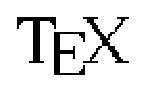
\includegraphics[height=0.75em]{./fig/xlatex.faconner.eps}}), 
voir\footnote{équivalent à taper la commande : \texttt{xdvi mon-document}.}
le résultat (bouton \fbox{\textsf{Visionner}}
ou \fbox{
\includegraphics[height=0.75em]{./fig/xlatex.visionner.eps}}), etc.

Lors de la compilation, en cas d'erreur, \LaTeX\ attend un ordre de
votre part. Les plus utiles sont :
\begin{itemize}
        \item[?] liste des commandes possibles ;

        \item[h] diagnostic détaillé et suggestion de solution ; 
 
        \item[q] arrêt de \LaTeX.
\end{itemize}

Pour avoir un descriptif plus étoffé des commandes \LaTeX\ 
utilisables, vous pouvez vous reporter à la documentation distribuée.
Si elle n'est pas suffisante, vous trouverez des informations
complémentaires à la bibliothèque dans \cite{lamport:latex:94} et
\cite{rolland:latex:95}.

Sous Solaris vous avez les lettres minuscules accentuées
accessibles directement par les raccourcis spéciaux \textsf{shift-F1 à F12}, 
et les majuscules par \textsf{CapsLock} puis \textsf{shift-F1 à F12}, 
ou bien plus classiquement par la séquence de touches 
\textsf{Compose accent lettre}.



\section{Titre de section}  

Ligne de remplissage pour visualiser la mise en page. Ligne de
remplissage pour visualiser la mise en page. 

\subsection{Titre de sous-section}
\subsubsection{Titre de sous-sous-section}
\paragraph{Titre de paragraphe}

Exemple de référence à une figure au format PostScript encapsulé
(figure~\ref{fig:exemple}). Cette figure a été créée à l'aide de
\texttt{xfig}\footnote{disponible sous Unix/Linux.} après exportation 
du fichier fig vers le format Encapsulated PostScript.

% Utilisation de la commande pour inclure un fichier eps
%------------------------------------------------------------------------------
%       \FigurePS{h,t,b,p}{largeur}{nom_fichier}{titre}{nom_symbolique} 
%------------------------------------------------------------------------------
% {h,t,b,p} donne l'ordre de préférence du positionnement de la figure :
%                 h -> here ; t -> top ; b -> bottom ; p -> end of part.
%           En général, ne pas modifier cet argument.

%------------------------------------------------------------------------------
\FigureEPS{h,t,b,p}{8.5cm}{./fig/exemple-figure.eps}
                  {Exemple d'inclusion d'une figure EPS}   
                  {fig:exemple}
%------------------------------------------------------------------------------

Pour inclure une image, on doit aussi la convertir en EPS, avec
la commande \texttt{convert}\footnote{
disponible aussi sous Unix/Linux et à privilégier 
car elle génère un EPS tout à fait standard 
(au contraire de nombreux pilotes Windows).}
\texttt{~image image.eps}, qui accepte pratiquement tous les formats d'images.


\subsection{Encore un titre de sous-section}

Exemple de liste à puces :
\begin{itemize}
        \item ligne de remplissage pour visualiser la mise en page. Ligne de
        remplissage pour visualiser la mise en page ;

        \item ligne de remplissage pour visualiser la mise en page. Ligne de
        remplissage pour visualiser la mise en page.
\end{itemize}

Ligne de remplissage pour visualiser la mise en page. Ligne de remplissage pour
visualiser la mise en page. 


\section{Conclusion} 
 
\LaTeX\ c'est facile pour produire des documents standard et nickel ! 
Et Bib\TeX\ pour les références, c'est le pied.

\bibliography{biblio}


\end{document}

%%%%%%%%%%%%%%%%%%%%%%%%%%%%%%%%%%%%%%%%%%%%%%%%%%%%%%%%%%%%%%%%%%%%%%%%%%%%%%%
